%!TEX TS-program = xelatex
%!TEX encoding = UTF-8 Unicode

\documentclass[
% -- opções da classe memoir --
12pt,				% tamanho da fonte
openright,			% capítulos começam em pág ímpar (insere página vazia caso preciso)
oneside,			% para impressão em recto e verso. Oposto a oneside
a4paper,			% tamanho do papel.
% -- opções da classe abntex2 --
% chapter=TITLE,		% títulos de capítulos convertidos em letras maiúsculas
% section=TITLE,		% títulos de seções convertidos em letras maiúsculas
% subsection=TITLE,	% títulos de subseções convertidos em letras maiúsculas
% subsubsection=TITLE,% títulos de subsubseções convertidos em letras maiúsculas
% -- opções do pacote babel --
% french,				% idioma adicional para hifenização
% spanish,			% idioma adicional para hifenização
brazil,				% o último idioma é o principal do documento
english,			% idioma adicional para hifenização
]{abntex2}
\RequireXeTeX %Force XeTeX check


% ---
% PACOTES
% ---

% ---
% Pacotes fundamentais
% ---
\usepackage{lmodern}			% Usa a fonte Latin Modern
\usepackage[T1]{fontenc}		% Selecao de codigos de fonte.
\usepackage[utf8]{inputenc}		% Codificacao do documento (conversão automática dos acentos)
\usepackage{indentfirst}		% Indenta o primeiro parágrafo de cada seção.
\usepackage{color}				% Controle das cores
\usepackage{graphicx}			% Inclusão de gráficos
\usepackage{microtype} 			% para melhorias de
% justificação
\usepackage{amsmath}
\usepackage{xltxtra}
% \setmainfont{Source Han Sans CN}
% \usepackage{xeCJK}
% ---
% \usepackage[UTF8]{ctex}
% \usepackage{xeCJK}
% \setCJKmainfont{SimSun}
% ---
% Pacotes de citações
%\usepackage{graphicx}
\usepackage{grffile}
\usepackage{longtable}
\usepackage{wrapfig}
\usepackage{rotating}
\usepackage[normalem]{ulem}
\usepackage{amsmath}
\usepackage{textcomp}
\usepackage{amssymb}
\usepackage{capt-of}
\usepackage{hyperref}
% \usepackage{xltxtra}
\usepackage{fontspec} %Font package
\usepackage{xunicode}
%Select fonts
% \setmainfont[Mapping=tex-text]{Hack Nerd Font}
% \setsansfont[Mapping=tex-text]{DroidSansMono Nerd Font}
% \setmonofont{Quivira}
\newfontfamily\uni[Mapping=tex-text]{Hack Nerd Font}
\newenvironment{uni}{\uni}{\par}
\DeclareTextFontCommand{\unifont}{\uni}
% Some unicode characters
% 
% \newcommand*{\uni}[1]{{\fontsize{12}{12}\fontfamily{}\selectfont \H{#1}}}

% \setmainfont{Source Han Sans CN}
\usepackage[brazilian,hyperpageref]{backref}	 % Paginas com as citações na bibl
\usepackage[alf]{abntex2cite}	% Citações padrão ABNT
\usepackage{graphicx}
\usepackage{graphics}

\usepackage{fontawesome5} % renderização de unicode
\usepackage{ucs}
% \usepackage{droid}
% \renewcommand{}{}
% \renewcommand{\ttfamily}{Symbols Nerd Font}
% \setmonofont{}
% ---
% Pacotes adicionais, usados no anexo do modelo de folha de identificação
% ---
% \usepackage{multicol}
% \usepackage{multirow}
% ---

% ---
% Pacotes adicionais, usados apenas no âmbito do Modelo Canônico do abnteX2
% ---
% \usepackage{lipsum}				% para geração de dummy text
% ---


% ---
% CONFIGURAÇÕES DE PACOTES
% ---

% Enumeração extendível
\usepackage{enumitem}
\setlist{nolistsep}

% Caminho dos arquivos-imagem
\graphicspath{
  {./Imagens/}
  {./Imagens/Linux}
  {./Imagens/WM}
  {./Imagens/BenchMarks}
  {./Imagens/Running}
}

% ---
% Configurações do pacote backref
% Usado sem a opção hyperpageref de backref
\renewcommand{\backrefpagesname}{Citado na(s) página(s):~}
% Texto padrão antes do número das páginas
\renewcommand{\backref}{}
% Define os textos da citação
\renewcommand*{\backrefalt}[4]{
  \ifcase #1 %
  Nenhuma citação no texto.%
  \or
  Citado na página #2.%
  \else
  Citado #1 vezes nas páginas #2.%
  \fi}%
% ---

% ---
% Informações de dados para CAPA e FOLHA DE ROSTO
% ---
\titulo{Free software in industry and academia}
\autor{PEDRO GOMES BRANQUINHO}
\orientador{Dr. Wei-Liang Qian}
\local{Lorena}
\data{2021}%
\instituicao{%
  University of São Paulo - USP \\
  Engineer School of Lorena
  \par
  Monograph, Conclusion Thesis
}%
\tipotrabalho{Dissertation}
% O preambulo deve conter o tipo do trabalho, o objetivo,
% o nome da instituição e a área de concentração
% Orientador: Prof. Dr. Ismael Maciel de
% Mancilha 
\preambulo{This monograph is presented to the Engineer School of Lorena, the University of São Paulo, so to be obtained the title of Barchelor by the Graduation Program on Engineering Physics with emphasis on the Science of Materials.}
% ---

% ---
% Configurações de aparência do PDF final

% alterando o aspecto da cor azul
\definecolor{blue}{RGB}{41,5,195}

% informações do PDF
\makeatletter
\hypersetup{
  % pagebackref=true,
  pdftitle={\@title},
  pdfauthor={\@author},
  pdfsubject={\imprimirpreambulo},
  pdfcreator={Pedro G. Branquinho},
  pdfkeywords={tese}{software}{livre},
  colorlinks=true,       		% false: boxed links; true: colored links
  linkcolor=blue,          	% color of internal links
  citecolor=blue,        		% color of links to bibliography
  filecolor=magenta,      		% color of file links
  urlcolor=blue,
  bookmarksdepth=4
}
\makeatother
% ---

% ---
% Espaçamentos entre linhas e parágrafos
% ---


% % O tamanho do parágrafo é dado por:
\setlength{\parindent}{0.8cm}

% % Controle do espaçamento entre um parágrafo e outro:
\setlength{\parskip}{0.2cm}  % tente também \onelineskip

% ---
% compila o indice
% ---
\makeindex
% ---

% ----
% Início do documento
% ----
\begin{document}
% Seleciona o idioma do documento (conforme pacotes do babel)
\selectlanguage{english}
% \selectlanguage{brazil}

% Retira espaço extra obsoleto entre as frases.
\frenchspacing

% ----------------------------------------------------------
% ELEMENTOS PRÉ-TEXTUAIS
% ----------------------------------------------------------
% \pretextual

% ---
% Capa
% ---
\imprimircapa
% ---

% ---
% Folha de rosto
% (o * indica que haverá a ficha bibliográfica)
% ---
\imprimirfolhaderosto*
% ---

% ---
% Inserir a ficha bibliografica
% ---

% Isto é um exemplo de Ficha Catalográfica, ou ``Dados internacionais de
% catalogação-na-publicação''. Você pode utilizar este modelo como referência. 
% Porém, provavelmente a biblioteca da sua universidade lhe fornecerá um PDF
% com a ficha catalográfica definitiva após a defesa do trabalho. Quando estiver
% com o documento, salve-o como PDF no diretório do seu projeto e substitua todo
% o conteúdo de implementação deste arquivo pelo comando abaixo:
%
% \begin{fichacatalografica}
%     \includepdf{fig_ficha_catalografica.pdf}
% \end{fichacatalografica}

\begin{fichacatalografica}
	\sffamily
	\vspace*{\fill}					% Posição vertical
	\begin{center}					% Minipage Centralizado
	\fbox{\begin{minipage}[c][8cm]{13.5cm}		% Largura
	\small
	\imprimirautor
	%Sobrenome, Nome do autor
	
	\hspace{0.5cm} \imprimirtitulo  / \imprimirautor. --
	\imprimirlocal, \imprimirdata-
	
	% \hspace{0.5cm} \thelastpage p. \\ %: il. (algumas color.) ; 30 cm.
	
	\hspace{0.5cm} \imprimirorientadorRotulo~\imprimirorientador\\
	
	\hspace{0.5cm}
	\parbox[t]{\textwidth}{\imprimirtipotrabalho~--~\imprimirinstituicao,
	\imprimirdata.}\\
	
	\hspace{0.5cm}
		1. Free Software.
		2. Open Source.
		2. Academy and Industry.
		I. Wei-Liang Qian.
		II. University EEL-USP.
		III. Escola de Engenharia de Lorena.
		IV. Free Software on Industry and Academia.
	\end{minipage}}
	\end{center}
      \end{fichacatalografica}
      \clearpage
% ---

% ---
% Dedicatória
% ---
\begin{dedicatoria}
   \vspace*{\fill}
   \centering
   \noindent
   \textit{To those whom found me in their own path\\
     and, by finding me, made part of my own.} \vspace*{\fill}
\end{dedicatoria}
% ---

% ---
% Agradecimentos
% ---
\begin{agradecimentos}

  My acknowledgments wouldn't fit in a single page. But, for the purpose of conciseness, I will mention those who are closer to my work. I thank first my advisor, Wei-Liang Qian, who in his patience and kindness knew how to conduce me to produce the present work. I thank Juan Zapata for the support and enthusiasm on teaching Mathematics and showing me the way of how to study it myself. Last but not least, I thank Luiz Eleno who has been a role-model for me, and has teach me so much about computing through out the years.

  And, in a big umbrella, I thank all those anonymous people who have contributed for my experience of communal sharing and understanding in the Open Source community. Specially, David Wilson, the founder of System's Crafter, from whom I derived the basis of my Emacs's system. 
  
\end{agradecimentos}
% ---

% % ---
% % Epígrafe
% % ---
% \begin{epigrafe}
%     \vspace*{\fill}
% 	\begin{flushright}
% 		\textit{``Não vos amoldeis às estruturas deste mundo, \\
% 		mas transformai-vos pela renovação da mente, \\
% 		a fim de distinguir qual é a vontade de Deus: \\
% 		o que é bom, o que Lhe é agradável, o que é perfeito.\\
% 		(Bíblia Sagrada, Romanos 12, 2)}
% 	\end{flushright}
% \end{epigrafe}
% % ---

% ---
% RESUMOS
% ---

% Abstract in English
\setlength{\absparsep}{18pt} % ajusta o espaçamento dos parágrafos do resumo
\begin{resumo}
  In this work, It's shown how to build a series of application only upon a Free Software system - EXWM, Artix Linux OSS. I explain how the experience of participating in the Open Community can be significant for other Engineers; specially Physics Engineers. It's delineated what are the current trends on the adoption of Free and/or Open Source Software (FOSS). Furthermore, I put forward some of the tools I used in Academia, and in Industry, and some other not so well known software, which could be used in these two contexts - e.g., Freqtrade, OR-Tools, Git(hub) et cetera. I also argue why Linux is such a key software for someone shifting to the Open Source paradigm.
  
 \textbf{Key-words}: trends. foss. academia. industry. linux. freqtrade. or-tools. git. github.
\end{resumo}

% Abstract (resumo) in Portuguese
\begin{resumo}[Resumo]
 \begin{otherlanguage*}{brazil}

  Demonstrou-se como é possível construir uma série de aplicações
  baseada em softwares de licença livre, à partir de um sistema
  aberto, o Linux com inteface EXWM - Emacs X Window Manager. Além
  disso, foi propiciado casos reais de aplicações na Indústria e no
  investimento privado, autônomo. Bem como, utilizações na Academia,
  à nível de lecionar, e pequisa. Sustenta-se que a economia aberta
  possui similaridade estrutural ao movimento \textit{Open Source} e
  seu desenvolvimento, o que aponta que essa é e continuará a ser,
  paulatinamente mais, o paradigma de desenvolvimento econômico
  tecnológico. Assim, imprescindível à formação do engenheiro.
  
   \vspace{\onelineskip}
  \noindent
  \textbf{Palavras-chaves}: software livre. automação. freqtrade. idústria. academia.
 \end{otherlanguage*}
\end{resumo}

% ---
% inserir lista de ilustrações
% ---
\pdfbookmark[0]{\listfigurename}{lof}
\listoffigures*
\cleardoublepage
% ---

% ---
% inserir lista de quadros
% ---
% \pdfbookmark[0]{\listofquadrosname}{loq}
% \listofquadros*
% \cleardoublepage
% ---

% ---
% inserir lista de tabelas
% ---
% \pdfbookmark[0]{\listtablename}{lot}
% \listoftables*
% \cleardoublepage
% ---

% ---
% inserir lista de abreviaturas e siglas
% ---
\begin{siglas}
  \item[FOSS] Free and Open Source Software  
  \item[abnTeX] ABsurdas Normas para TeX
\end{siglas}
% ---

% % ---
% % inserir lista de símbolos
% % ---
% \begin{simbolos}
%   \item[$ \Gamma $] Letra grega Gama
%   \item[$ \Lambda $] Lambda
%   \item[$ \zeta $] Letra grega minúscula zeta
%   \item[$ \in $] Pertence
% \end{simbolos}
% % ---

% ---
% inserir o sumario
% ---
\pdfbookmark[0]{\contentsname}{toc}
\tableofcontents*
\cleardoublepage
% ---



% ----------------------------------------------------------
% ELEMENTOS TEXTUAIS
% ----------------------------------------------------------
\textual

% ----------------------------------------------------------
% Introdução (exemplo de capítulo sem numeração, mas presente no Sumário)
% ----------------------------------------------------------

\chapter[Introduction]{Introduction}
% \addcontentsline{toc}{chapter}{Introdução}

In training a Physics Engineer, of which, by definition, is a generalist professional. The use of Free and Open Sourced Softwares (FOSS), as well as the participation in the Open Source community (OS), are two detrimental experiences to have.
% Na formação de um engenheiro físico, o qual, por definição, é um profissional generalista, os softwares abertos (FOSS - Free and Open Source Software) e a participação da comunidade Open Source (OS) são detrimentais para sua formação.

The variability, which open source software (OSS) brings to existence of applications and it's extension, can change altogether user's experience. Thus, taking him closer to acting as a developer. This experience of interloping user and developer roles doesn't require that you are a computer scientist or a Information Technology (IT) professional by training. For, programming can be seen as both a Science and an Art \cite{knuth1968art} - e.g., an exercise of self-expression.
% A diversidade os quais softwares extensíveis acarretam (\autoref{sec:diversidade}) podem mudar completamente a experiência do usuário, e o trazer mais próximo do papel de desenvolvedor. Essa experiência não necessita de ser exclusiva de cientistas da computação ou profissionais de TI. Pois, a programação pode ser encarada tanto como ciência e arte \cite{knuth1968art}.

OSS guarantees four fundamental liberties \autoref{sec:opensource}, the right to study, copy, modify and redistribute it.
% Os Softwares Abertos possuem quatro liberdades pétreas \autoref{sec:opensource}, garantindo os direitos de estudo, cópia, modificação e redistribuição.

Just as the scientific enterprise benefits, with it's rapid development, by means of the global community's participation, which holds space for individuals with a variety of different training. Also, the computation enterprise benefits from the variety of people's training, which constitute the body of the open source community.
% Bem como a ciência se beneficia com seus rápidos avanços, de uma comunidade global de participantes, com as mais distintas especializações profissionais. Também, beneficia-se a computação com a comunidade aberta, e especialização eclética, tanto de membros quanto de softwares.

\chapter{Bibliography review}
\section{Open Source}
\label{sec:opensource}

Any program which permits the user-developer to have the following liberties:
\begin{enumerate}
\item The right to run the program, as seen fit, for any end.
  % Direito de rodar o programa, como você desejar, para qualquer fim.
\item The right to access the source code and study it.
  % Direito ao acesso ao código-fonte, para estudá-lo.
\item The right to copy and redistribute it.
  % Direito de cópia e distribuição.
\item The right to modify the software.
\end{enumerate}

% Qualquer programa que permita o usuário-programador ter as seguintes
% liberdades:

% \begin{enumerate}
% \item Direito de rodar o programa, como você desejar, para qualquer fim.
% \item Direito ao acesso ao código-fonte, para estudá-lo.
% \item Direito de cópia e distribuição.
% \item Direito à modificação do software.
% \end{enumerate}

Practically, the Open Source community fundamentally base itself upon
the free distribution of it's tools and programs. One of the differential
advantage of having innumerable other people extending the same
software is that the advancement of the frontier of the program, in
many directions, increases rapidly in relation to a program controlled
by a limited number of programmers.

% De maneira prática, a comunidade Open Source, fundamentalmente, se
% baseia no compartilhamento de suas configurações. As vantagens de
% existirem inúmeras outras pessoas utilizando o mesmo software é de
% que a melhoria da fronteira do programa é expandida de forma
% acrescida, em comparação a de um time restrito de usuários.

\subsection{Diversity}
\label{sec:diversity}

Given that one fundamental right of OSS is the modification and
propagation of new modified versions. This right implies in the
observable wide range of maintained versions of these software, which
doesn't have a parallel in any other technological enterprise. 
% Dado que um direito fundamental dos softwares livres é a modificação e propagação das versões modificadas, existe uma diversidade de expressividade, sem paralelos em outras áreas da tecnologia.

For an example, one key application in any user's computer is a general
Graphical User Interface (GUI)'s manager, commonly known as Window
Manager (WM). These can be both Floating or Tilling, or mixed WM,
e.g., Floating WM are those that the user must hover windows and
adjust them manually; Tilling WM are those that a pre-defined program
have a set of rules to resize automatically the windows in a screen.

% Por exemplo, uma parte de software fundamental na configuração de um computador é seu gerenciador de interfaces (Window Manager). Onde, um programa é devotado a gerenciar como outros programas gráficos devem se dispor na tela de computador.

While private Operational Systems (OS), as Windows and MacOS, have
frequent releases - a total of twenty five releases for
Windows. Generally, they've few \textit{active} versions; Windows have
currently four \cite{wikipedia_2021W}. MacOS also have four active
versions \cite{wikipedia_2021Mac}.
% Enquanto sistemas operacionais (Operational Systems) privados, como Windows e MacOS possuem versões lançadas frequentemente - vinte e cinco versões lançadas de Windows. O Windows possui apenas quatro versões, com suporte ativo \cite{wikipedia_2021W}.

% São vinte lançamentos de MacOS, e quatro verões mantidas \cite{wikipedia_2021Mac}.

The fact there are only narrowly supported versions is due to, among
many contributing factors, users lack the right to alter and extend
the software's behavior. Therefore, they fall victims of discontinued
support and restrictive access to the company's official upgrades. 
% Essa estreiteza de versões se dá, dentre os fatores, pois os usuários são cerciados do direito de extender ou alterar os comportamentos programados no sistema. Assim, vítimas do suporte descontinuado e de sua atualização de versões restritivas.

On the other hand, there exists, in parallel, around two hundred
seventy eight available distributions of Linux
\cite{wikipedia_2021Linux}. Of which, there are main/root
distributions, which each embody a set of different principles; theoretical and practical philosophies of how to extend software.  
% Em contra partida, existem, paralelamente, por volta de 278 distribuições de Linux \cite{wikipedia_2021Linux}. Onde, existem as distribuições raízes, com princípios e filosofias de desenvolvimentos teóricos e práticos diferentes.

Thus, just as with any other scope of software, the variability of
FOSS always will be grater than monopolized ones.
% Assim, bem como em qualquer outro escopo de software, a variação dos softwares abertos e livres (FOSS) sempre serão superiores aos monopolizados.

\section{GNU/Linux}
There are root distributions of Linux, from which many other
distributions emanate. Generically, these partitions are called
families. We cite some of the most influential and popular ones, Red
Hat Linux (\faIcon{redhat}), Debian (\unifont{}), CentOS
(\faIcon{centos}), Fedora(\faIcon{fedora}), Pacman-based
(\unifont{}/\unifont{}), OpenSUSE (\faIcon{suse}),
Gentoo-based (\unifont{}), Ubuntu-based(\faIcon{ubuntu}),
Slackware (\unifont{}), Open Sourced-based and the
Independent Distributions (\unifont{}/\faIcon{linux}).

\begin{figure}[!htb]
  \caption{\label{fig:linux-genealogy} Genealogy of Linux's Distributions}
  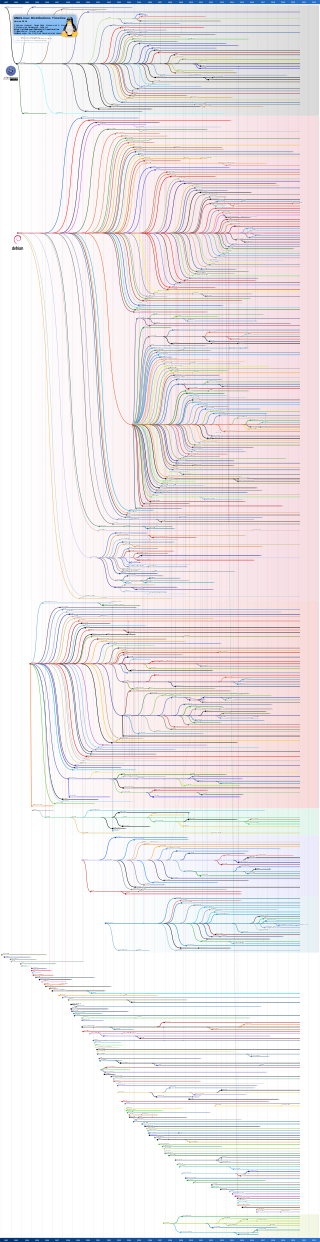
\includegraphics[height=\textwidth, angle=-90]{diversidade}
  \legend{Genealogical history of Linux Distributions \cite{wikipedia_2021Linux}}
  % \legend{Histórico de evolução das distribuições Linux \cite{wikipedia_2021Linux}}
\end{figure}

\bibliography{bib}
\end{document}
